% This file was created by matlab2tikz.
%
%The latest updates can be retrieved from
%  http://www.mathworks.com/matlabcentral/fileexchange/22022-matlab2tikz-matlab2tikz
%where you can also make suggestions and rate matlab2tikz.
%
\definecolor{mycolor1}{rgb}{0.00000,0.44700,0.74100}%
\definecolor{mycolor2}{rgb}{0.92900,0.69400,0.12500}%
\definecolor{mycolor3}{rgb}{0.46600,0.67400,0.18800}%
\definecolor{mycolor4}{rgb}{0.63500,0.07800,0.18400}%
\definecolor{mycolor5}{rgb}{0.85000,0.32500,0.09800}%
%
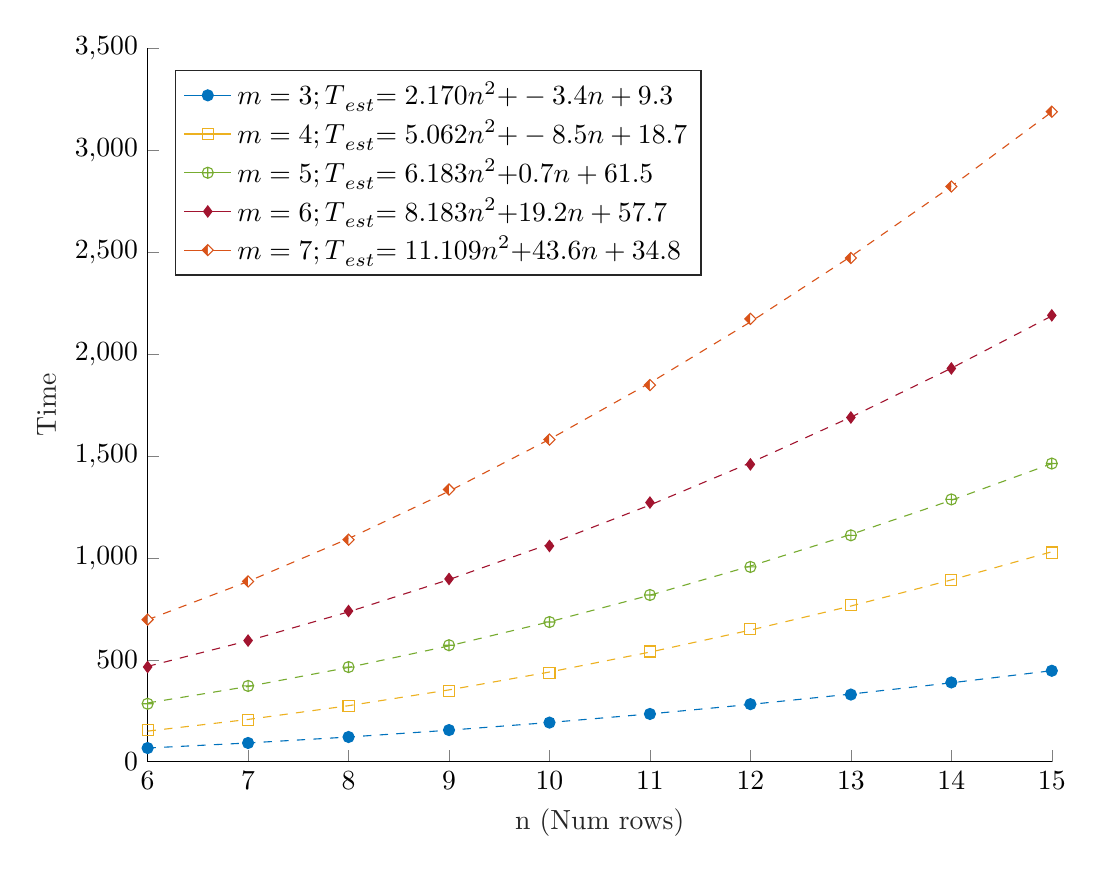
\begin{tikzpicture}

\begin{axis}[%
width=4.521in,
height=3.566in,
at={(0.758in,0.481in)},
scale only axis,
xmin=6,
xmax=15,
xlabel style={font=\color{white!15!black}},
xlabel={n (Num rows)},
ymin=0,
ymax=3500,
ylabel style={font=\color{white!15!black}},
ylabel={Time},
axis background/.style={fill=white},
title style={font=\bfseries},
% title={$\text{Average ticks until solution as a function of n. On n }\times\text{ m grid. (k = 3)}$},
axis x line*=bottom,
axis y line*=left,
legend style={at={(0.03,0.97)}, anchor=north west, legend cell align=left, align=left, draw=white!15!black}
]
\addplot [color=mycolor1, draw=none, mark=*, mark options={solid, mycolor1}]
  table[row sep=crcr]{%
6	66.874\\
7	91.86\\
8	121.156\\
9	155.144\\
10	191.816\\
11	234.246\\
12	282.3\\
13	329.44\\
14	388.884\\
15	446.218\\
};
\addlegendentry{$\text{m = 3; T}_{\text{est}}\text{ =  2.170n}^\text{2}\text{ + -3.4n +  9.3}$}

\addplot [color=mycolor1, dashed, forget plot]
  table[row sep=crcr]{%
6	67.053563636361\\
7	91.8672727272717\\
8	121.020860606061\\
9	154.514327272728\\
10	192.347672727274\\
11	234.520896969698\\
12	281.034000000001\\
13	331.886981818182\\
14	387.079842424242\\
15	446.61258181818\\
};
\addplot [color=mycolor2, draw=none, mark=square, mark options={solid, mycolor2}]
  table[row sep=crcr]{%
6	154.3\\
7	206.298\\
8	272.258\\
9	347.434\\
10	436.504\\
11	540.682\\
12	650.282\\
13	768.704\\
14	891.216\\
15	1026.388\\
};
\addlegendentry{$\text{m = 4; T}_{\text{est}}\text{ =  5.062n}^\text{2}\text{ + -8.5n + 18.7}$}

\addplot [color=mycolor2, dashed, forget plot]
  table[row sep=crcr]{%
6	150.015690909087\\
7	207.32878181818\\
8	274.765372727273\\
9	352.325463636365\\
10	440.009054545456\\
11	537.816145454547\\
12	645.746736363638\\
13	763.800827272728\\
14	891.978418181817\\
15	1030.27950909091\\
};
\addplot [color=mycolor3, draw=none, mark=oplus, mark options={solid, mycolor3}]
  table[row sep=crcr]{%
6	284.328\\
7	371.772\\
8	464.396\\
9	571.52\\
10	685.282\\
11	818.122\\
12	955.776\\
13	1110.83\\
14	1287.138\\
15	1463.198\\
};
\addlegendentry{$\text{m = 5; T}_{\text{est}}\text{ =  6.183n}^\text{2}\text{ +  0.7n + 61.5}$}

\addplot [color=mycolor3, dashed, forget plot]
  table[row sep=crcr]{%
6	288.106381818179\\
7	369.160563636363\\
8	462.580245454545\\
9	568.365427272728\\
10	686.51610909091\\
11	817.032290909092\\
12	959.913972727274\\
13	1115.16115454546\\
14	1282.77383636364\\
15	1462.75201818182\\
};
\addplot [color=mycolor4, draw=none, mark=diamond*, mark options={solid, mycolor4}]
  table[row sep=crcr]{%
6	464.716\\
7	594.304\\
8	739.322\\
9	896.734\\
10	1058.702\\
11	1271.748\\
12	1459.24\\
13	1689.216\\
14	1929.714\\
15	2190.392\\
};
\addlegendentry{$\text{m = 6; T}_{\text{est}}\text{ =  8.183n}^\text{2}\text{ + 19.2n + 57.7}$}

\addplot [color=mycolor4, dashed, forget plot]
  table[row sep=crcr]{%
6	467.728399999988\\
7	593.345781818177\\
8	735.330012121213\\
9	893.681090909095\\
10	1068.39901818182\\
11	1259.4837939394\\
12	1466.93541818182\\
13	1690.75389090909\\
14	1930.93921212121\\
15	2187.49138181817\\
};
\addplot [color=mycolor5, draw=none, mark=halfsquare left*, mark options={solid, mycolor5}]
  table[row sep=crcr]{%
6	697.354\\
7	884.39\\
8	1089.346\\
9	1335.698\\
10	1580.916\\
11	1848.156\\
12	2173.03\\
13	2471.96\\
14	2822.684\\
15	3189.696\\
};
\addlegendentry{$\text{m = 7; T}_{\text{est}}\text{ = 11.109n}^\text{2}\text{ + 43.6n + 34.8}$}

\addplot [color=mycolor5, dashed, forget plot]
  table[row sep=crcr]{%
6	696.495945454542\\
7	884.544987878786\\
8	1094.81122727273\\
9	1327.29466363636\\
10	1581.9952969697\\
11	1858.91312727273\\
12	2158.04815454546\\
13	2479.40037878788\\
14	2822.9698\\
15	3188.75641818182\\
};
\end{axis}
\end{tikzpicture}%
